\section{The Six Trigonometric Functions}
\noindent\textbf{Central question.} How do six functions arise naturally from the same moving point on a circle?

\subsection{From a point to six functions}
Last week we studied the unit-circle point $P=(x,y)=(\cos\theta,\sin\theta)$. The two coordinates determine four additional ratios whenever the denominators are nonzero:
\[
\begin{aligned}
\sin\theta&=y,& \cos\theta&=x,&
\tan\theta&=\frac{y}{x},\\
\csc\theta&=\frac1y,& \sec\theta&=\frac1x,&
\cot\theta&=\frac{x}{y}.
\end{aligned}
\]
These are not six unrelated measurements. They are six different ways of reading the same geometric information.

\begin{definition}The \emph{tangent} function is $\tan\theta=\sin\theta/\cos\theta$ where $\cos\theta\neq0$. The functions $\csc,\sec,\cot$ are the reciprocals of $\sin,\cos,\tan$ respectively, wherever defined.\end{definition}

\begin{example}At $\theta=\pi/3$ the circle point is $(1/2,\sqrt3/2)$. Thus $\tan\theta=\sqrt3$, $\sec\theta=2$, $\csc\theta=2/\sqrt3=2\sqrt3/3$, and $\cot\theta=1/\sqrt3=\sqrt3/3$.\end{example}

\subsection{Signs and the quadrants}
The coordinate signs determine every trig-function sign. In quadrant I both coordinates are positive; in II, only sine is positive; in III, tangent is positive because both coordinates are negative; and in IV, only cosine is positive. Reciprocal functions have the same signs as their corresponding original functions.

\begin{example}For $\theta=5\pi/4$, the reference angle is $\pi/4$ and $P=(-\sqrt2/2,-\sqrt2/2)$. Therefore $\tan\theta=1$, $\sec\theta=-\sqrt2$, and $\csc\theta=-\sqrt2$.\end{example}

\subsection{Where are the functions undefined?}
Division by zero has no meaning. In particular, $\tan\theta$ and $\sec\theta$ do not exist where $\cos\theta=0$, at $\pi/2+k\pi$. Similarly $\cot\theta$ and $\csc\theta$ do not exist where $\sin\theta=0$, at $k\pi$, for any integer $k$. The word \emph{undefined} matters: an undefined value is not the number zero.

\begin{practice}Find all six trig-function values at $\theta=3\pi/2$, identifying every undefined value.\end{practice}

\subsection{Right triangles are a special case}
For an acute angle $\theta$ in a right triangle, scale the triangle so its hypotenuse has length $1$. The opposite and adjacent sides then give the coordinates $\sin\theta$ and $\cos\theta$. Restoring a general hypotenuse $h$ gives
\[
\sin\theta=\frac{\text{opposite}}{h},\quad
\cos\theta=\frac{\text{adjacent}}{h},\quad
\tan\theta=\frac{\text{opposite}}{\text{adjacent}}.
\]
The unit circle is more general than the right-triangle definitions: it handles negative angles, obtuse angles, and angles exceeding a full revolution.

\begin{example}A ramp rises $1.5$ meters over a horizontal run of $6$ meters. Its angle of inclination satisfies $\tan\theta=1.5/6=1/4$. Therefore $\theta=\arctan(1/4)\approx14.0^\circ$.\end{example}

\subsection{Special angles without memorizing a disconnected table}
An equilateral triangle of side $2$ splits into two right triangles with sides $1,\sqrt3,2$. This produces $\sin30^\circ=1/2$ and $\cos30^\circ=\sqrt3/2$. A square of side $1$ has diagonal $\sqrt2$, producing $\sin45^\circ=\cos45^\circ=\sqrt2/2$.

\begin{center}
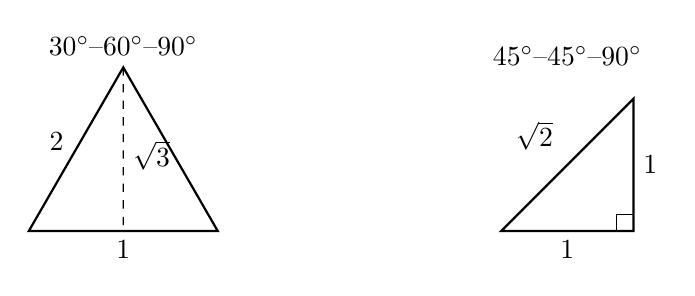
\begin{tikzpicture}[scale=1.2]
\coordinate(A)at(0,0);\coordinate(B)at(2,0);\coordinate(C)at(1,1.732);
\draw[thick](A)--(B)--(C)--cycle;\draw[dashed](C)--(1,0);
\node[below]at(1,0){$1$};\node[left]at(.47,.95){$2$};\node[right]at(1,0.8){$\sqrt3$};
\node[above]at(1,1.75){$30^\circ$--$60^\circ$--$90^\circ$};
\begin{scope}[xshift=5cm]
\draw[thick](0,0)--(1.4,0)--(1.4,1.4)--cycle;
\draw(1.22,0)rectangle(1.4,.18);
\node[below]at(.7,0){$1$};\node[right]at(1.4,.7){$1$};\node[above left]at(.65,.75){$\sqrt2$};
\node[above]at(.7,1.65){$45^\circ$--$45^\circ$--$90^\circ$};
\end{scope}\end{tikzpicture}
\end{center}

\subsection{Applications: orientation and measurement}
Suppose an observer stands $40$ m from the foot of a vertical tower. The angle of elevation to its top is $35^\circ$. The tower's height $h$ satisfies
\[
\tan35^\circ=\frac{h}{40},\qquad h=40\tan35^\circ\approx28.0\text{ m}.
\]
Here the tangent function links an angle to a ratio of lengths. Always sketch the physical situation and label which distances are opposite and adjacent before calculating.

\subsection{Exercises}
\begin{enumerate}
\item At $\theta=2\pi/3$, find all six functions exactly.
\item At $\theta=7\pi/4$, find $\tan,\cot,\sec,\csc$.
\item Explain geometrically why $\tan(\pi/2)$ is undefined.
\item For which angles in $[0,2\pi)$ is $\csc\theta$ undefined?
\item A right triangle has opposite side $5$ and adjacent side $12$. Find all six trig ratios exactly.
\item A ladder leans against a wall, reaching $8$ m high. Its foot is $3$ m from the wall. Find the angle with the ground.
\item A drone is viewed at an elevation angle of $28^\circ$ from a point $75$ m horizontally from the point below it. Estimate its altitude.
\item Show that $\sin^2\theta+\cos^2\theta=1$ implies $1+\tan^2\theta=\sec^2\theta$ wherever $\cos\theta\neq0$.
\end{enumerate}
\clearpage
